
\subsection{Data layer}

\subsubsection{Requirements}

\subsubsection{Schema}

    \begin{figure}[!ht]
        \centering
        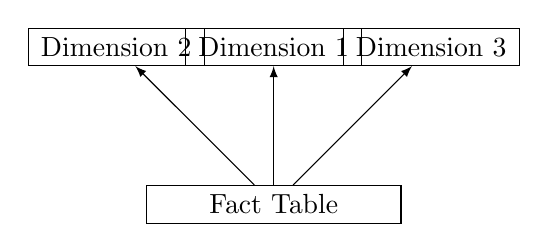
\begin{tikzpicture}[node distance=2cm]
            \node (fact) [draw, text width=3cm, align=center] {Fact Table};
            \node (dim1) [draw, text width=2cm, align=center, above of=fact] {Dimension 1};
            \node (dim2) [draw, text width=2cm, align=center, left of=dim1] {Dimension 2};
            \node (dim3) [draw, text width=2cm, align=center, right of=dim1] {Dimension 3};
        
            \draw [-latex] (fact) -- (dim1);
            \draw [-latex] (fact) -- (dim2);
            \draw [-latex] (fact) -- (dim3);
        \end{tikzpicture}
        \caption{Database schema}
        \label{fig:Database schema}
    \end{figure}
\subsection{Middle layer}

The middle layer, also known as the business logic layer, is an optional layer that sits between the server and data layers. This layer is responsible for processing the client requests and generating responses, and it can implement additional application logic beyond what is implemented in the server layer. In a WMS, the middle layer can be used to implement additional business logic, such as complex inventory management, order routing, or shipping optimization. The middle layer can be composed of various technologies, such as message brokers, API gateways, or microservices.

\subsection{Server layer}

The server layer, also known as the application layer, is the layer that processes the client requests and generates responses. This layer is responsible for implementing the application's business logic and managing the application's resources. The server layer can be composed of one or more servers, and it can use various technologies, such as web servers, application servers, or messaging servers. In a WMS, the server layer is responsible for processing warehouse operations, managing inventory, and optimizing warehouse processes.

\subsection{Client layer}

The client layer or presentation layer is the layer of the WMS that interacts with the end-user. This layer is responsible for presenting the application's user interface (UI) to the user and processing user input. The client layer can be composed of various technologies, such as web browsers, desktop applications, or mobile apps. In a WMS, the client layer enables the users to access the system and interact with it to perform operations such as inventory management, order processing, and shipping.
